\section{Network Blueprint}
\subsection{Recommended Equipment}
The following choice of hardware is based on the devices available in Cisco Packet Tracer.
\subsubsection{Router: CISCO2911/K9 }
\begin{itemize}
    \item Quantity: 3
    \item Specification: 3 Gigabit Ethernet Port, 4 Serial Port, 4 Fast Ethernet Port
    \item Ethernet connects the switches and routers in the same area
    \item Serial connects to devices in other areas
\end{itemize}
\begin{figure}[H]
    \centering
    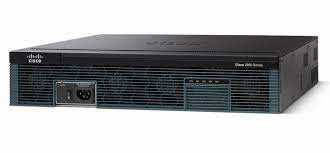
\includegraphics[width=0.6\textwidth]{./assets/router.png}
    \caption{Router CISCO2911/K9}
\end{figure}

\subsubsection{Switches: 2960 24TT}
\begin{itemize}
    \item Quantity: 17
    \item Specification: 24 Fast Ethernet Port, 2 Gigabit Ethernet Port
    \item To provide the DHCP services, each headquarter or branch will need 1 switch
    \item For headquarter, we need 5 switches for 100 workstations
    \item For branches, we need 3 switches for each branch correspond to 50 workstations
    \item A switch at each branch or headquarter to connect the servers to router
\end{itemize}

\begin{figure}[H]
    \centering
    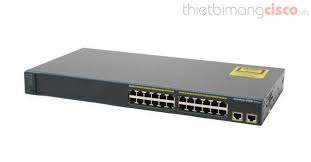
\includegraphics[width=0.7\textwidth]{./assets/switch.png}
    \caption{Switch 2960 24TT}
\end{figure}

\subsubsection{Access point: WRT300N}
\begin{itemize}
    \item Quantity: 3
    \item Specification: 2.4GHz channel WPA2-PSK built-in DHCP server

    \item Provide wireless connection through WPA-PSK authentication
\end{itemize}

\begin{figure}[H]
    \centering
    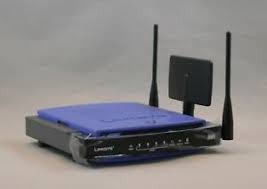
\includegraphics[width=0.5\textwidth]{./assets/wireless_router.png}
    \caption{Access point WRT 300N}
\end{figure}

\subsubsection{DHCP Server}
\begin{itemize}
    \item Quantity: 3
    \item Specification: Static IP procide DHCP service.
\end{itemize}

\subsubsection{Server}
\begin{itemize}
    \item Quantity: 11
    \item Specification: 5 servers for Headquarter, 3 for each branch
\end{itemize}

\subsubsection{Cables}
\begin{figure}[H]
    \centering
    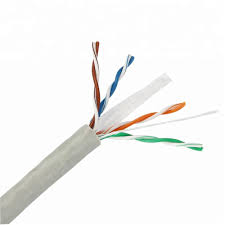
\includegraphics[width=0.4\textwidth]{./assets/copper.png}
    \caption{Straight-through copper cable}
\end{figure}

\begin{figure}[H]
    \centering
    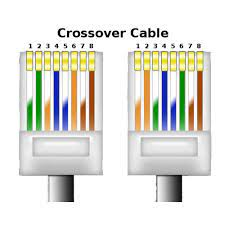
\includegraphics[width=0.4\textwidth]{./assets/crossover.png}
    \caption{Crossover copper cable}
\end{figure}

\begin{figure}[H]
    \centering
    
\includegraphics[width=0.6\textwidth]{./assets/lease.png}
    \caption{Leased line cable}
\end{figure}

\subsection{IP Address Table}
\subsubsection{Headquarter}
\begin{center}
  \begin{tabular}{|p{0.06\textwidth}|p{0.2\textwidth}|p{0.15\textwidth}|p{0.15\textwidth}|p{0.15\textwidth}|}
  \hline
   VLAN & Dept & Network ID & Default Gateway & Internet side IP\\
   \hline
   10 & IT/Work Station & 10.0.10.0/24 & 10.0.10.1/24 & 200.0.0.1/30 \\
   \hline
   50 & IT/Server & 10.0.50.0/24 & 10.0.50.1/24 & 200.0.0.1/30\\
   \hline
   N.A & IT/Wireless & 192.168.0.0/24 & 192.168.0.1/24 & 10.0.1.2/30\\
   \hline
    N.A & HQ Gateway router - Wireless Router
&10.0.1.0/30
&10.0.1.1/30
&200.0.0.1/30
\\
\hline
N.A & HQ Gateway router serial link 0
&10.0.0.1/30
&N.A
&N.A\\
\hline
N.A & HQ Gateway router serial link 1
&10.0.0.5/30
&N.A
&N.A
\\
\hline
   \end{tabular}
\end{center}
\subsubsection{Nha Trang branch}
\begin{center}
  \begin{tabular}{|p{0.06\textwidth}|p{0.2\textwidth}|p{0.15\textwidth}|p{0.15\textwidth}|p{0.15\textwidth}|}
  \hline
   VLAN & Dept & Network ID & Default Gateway & Internet side IP\\
   \hline
   10 & IT/Work Station
&10.1.10.0/24
&10.1.10.1/24
&200.0.1.1/30
 \\
 \hline
 50 & IT/Server
&10.1.50.0/24
&10.1.50.1/24
&200.0.1.1/30
\\
\hline
N.A &     IT/Wireless
&192.168.0.0/24
&192.168.0.1/24
&10.1.1.2/30
\\
\hline
N.A & NT Gateway router - Wireless Router
&10.1.1.0/30
&10.1.1.1/30
&200.0.1.1/30
\\
\hline
N.A & NT Gateway router serial link 0
&10.0.0.2/30
&N.A
&N.A
\\
\hline
   \end{tabular}
\end{center}

\subsubsection{Da Nang branch}
\begin{center}
  \begin{tabular}{|p{0.06\textwidth}|p{0.2\textwidth}|p{0.15\textwidth}|p{0.15\textwidth}|p{0.15\textwidth}|}
  \hline
   VLAN & Dept & Network ID & Default Gateway & Internet side IP\\
   \hline
   10 & IT/Work Station
&10.2.10.0/24
&10.2.10.1/24
&200.0.2.1/30
 \\
 \hline
 50 & IT/Server
&10.2.50.0/24
&10.2.50.1/24
&200.0.2.1/30
\\
\hline
N.A &     IT/Wireless
&192.168.0.0/24
&192.168.0.1/24
&10.2.1.2/30
\\
\hline
N.A & NT Gateway router - Wireless Router
&10.2.1.0/30
&10.2.1.1/30
&200.0.2.1/30
\\
\hline
N.A & NT Gateway router serial link 0
&10.0.0.6/30
&N.A
&N.A
\\
\hline
   \end{tabular}
\end{center}